\documentclass[12pt,fleqn]{article}\usepackage{../../common}
\begin{document}
Simulasyon

Önce basit bir simülasyon kodlayalım. Bazı toplar var, onları başta bir kuvvetle
rasgele yönlere iteceğiz ve ne yapacaklarına bakacağız. Fiziksel parametreler
şöyle, yerçekimi sabiti $g = 0.8$ (dünyadan daha az), topların birbirine ya da
duvara çarpması sonucu hiç enerji kaybı olmuyor.

Bu tür bir sistemin konumu, o anki hali her parçacık için bazı değişkenlerin
takip edilmesiyle olacak, bu değişkenler pozisyon, hız, kuvvet. Kütle her
parçacık için aynı olacak.

Parçacık hareketi o parçacık üzerinde uygulanan kuvvet ile belirlenir, Newton
denklemi $m \bar{a} = \bar{f}$, ki ivme ve kuvvet çok boyutlu dikkat edelim, o
sebeple vektör notasyonu olarak üstte çizgi kullandık. Peki ivmeden, hiza ve yer
değişikliğine nasıl gideriz? Newton formülünü bir ODE olarak tekrar düzenlersek
onu ileri doğru entegre edebiliriz. Yer $\bar{x}$, hız $\bar{v}$ olmak üzere
[5,6] ve her $i$ parçacığı için,

$$
\dot{\bar{v}}_i = \bar{f}_i / m_i
$$

$$
\dot{\bar{x}}_i = \bar{v}_i
$$

Bu tür bir sistemi entegre etmek için Euler'in metotu kullanılabilir [5, sf 5],
her $n$ anında bir sonraki $n+1$ değeri için

$$
\bar{x}^{n+1} = \bar{x}^n + h \bar{v}^n
$$

$$
\bar{v}^{n+1} = \bar{v}^n + h \bar{a}^n
$$

ki $h$ ufak zaman aralığı olarak alınır, bir diğer isim $\Delta t$ olabilir,
alttaki kodda \verb!dt! . O zaman her zaman diliminde her parçacığa etki eden
kuvvetler toplanır, bir nihai kuvvet vektörü elde edilir. Ardından üstteki
formüllerle sistem her parçacık için entegre edilir ve bir sonraki sistem durumu
elde edilir.

Bu ilk sistemde bazı basitleştirmeler var; kuvvet uygulanma ve onun hıza
dönüşmesine her koşulda bakmıyoruz, duvarlar ve parçacıklar arası etkileri direk
hız üzerinde uyguluyoruz. Topların birbirine çarpma sonucu hız vektörlerinin
hesabı [4]'te.

Kodlama notu, çarpışma hesabı için her parçacığın diğer parçacığa yakınlık
kontrolü pahalı olursa, daha fazla parçacık için mesela, bunun için böleç
tekniği kullanılabilir [3].

Genel grafik yöntemi şurada [1] işlendi.

\inputminted[fontsize=\footnotesize]{python}{sim.py}


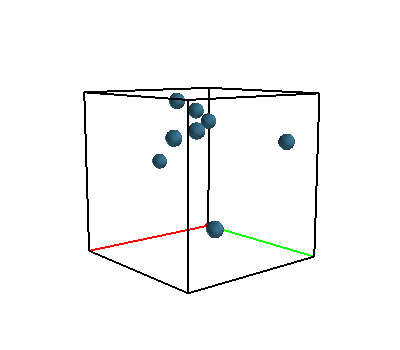
\includegraphics[width=15em]{glutout-140.png}
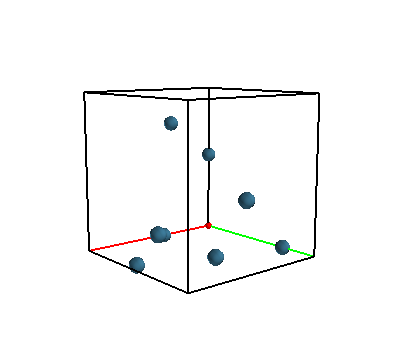
\includegraphics[width=15em]{glutout-390.png}

Tüm resimleri birleştirirsek,

\begin{minted}[fontsize=\footnotesize]{python}
convert -scale 30% /tmp/glutout-*.png /tmp/balls1.gif
\end{minted}

Sonuç [2]'de görülebilir.


Kaynaklar

[1] Bayramlı, {\em OpenGL, PyOpenGL}, \url{https://burakbayramli.github.io/dersblog/sk/2020/08/pyopengl.html}

[2] Bayramlı, {\em Simulasyon 1 Animasyon},
    \url{https://github.com/burakbayramli/classnotes/blob/master/phy/phy_007_sim/balls1.gif?raw=true}

[3] Bayramlı, {\em Bilgisayar Bilim, Geometrik Anahtarlama (Spatial Hashing) ve Izgara (Grid) ile En Yakın Noktaları Bulmak}

[4] Bayramlı, Fizik, {\em Temel Fizik 2, Dönüşler, Basınç, Çarpışma}

[5] Müller, {\em Fluid Simulation SIGGRAPH 2007 Course Notes},

[6] {\em Visual Interactive Simulation (Spring 15)},
    \url{https://www8.cs.umu.se/kurser/5DV058/VT15/}

\end{document}
